This section focuses on introducing the proposed unsupervised hyperspectral image segmentation algorithm, Adaptive Superpixel Cuts for Hyperspectral Images (ASC-HSI). This segmentation algorithm for hyperspectral images presents a two-stage approach that addresses challenges in hyperspectral data analysis. Unlike traditional methods that operate directly on every pixel, this algorithm leverages a clever step of pre-segmenting the image into small, uniform regions called superpixels. This initial segmentation based on spectral similarity offers a significant runtime advantage. By focusing on these superpixels instead of individual pixels, the algorithm reduces the computational complexity involved in subsequent processing stages. The second stage refines the segmentation by incorporating the estimated abundance of different materials within each superpixel region. This combination of efficient superpixel processing and material abundance estimation offers potential advantages in accuracy, particularly for handling mixed pixels and spectrally similar materials in distinct locations

% \begin{figure}[h]
%     \centering % This centers the image
%     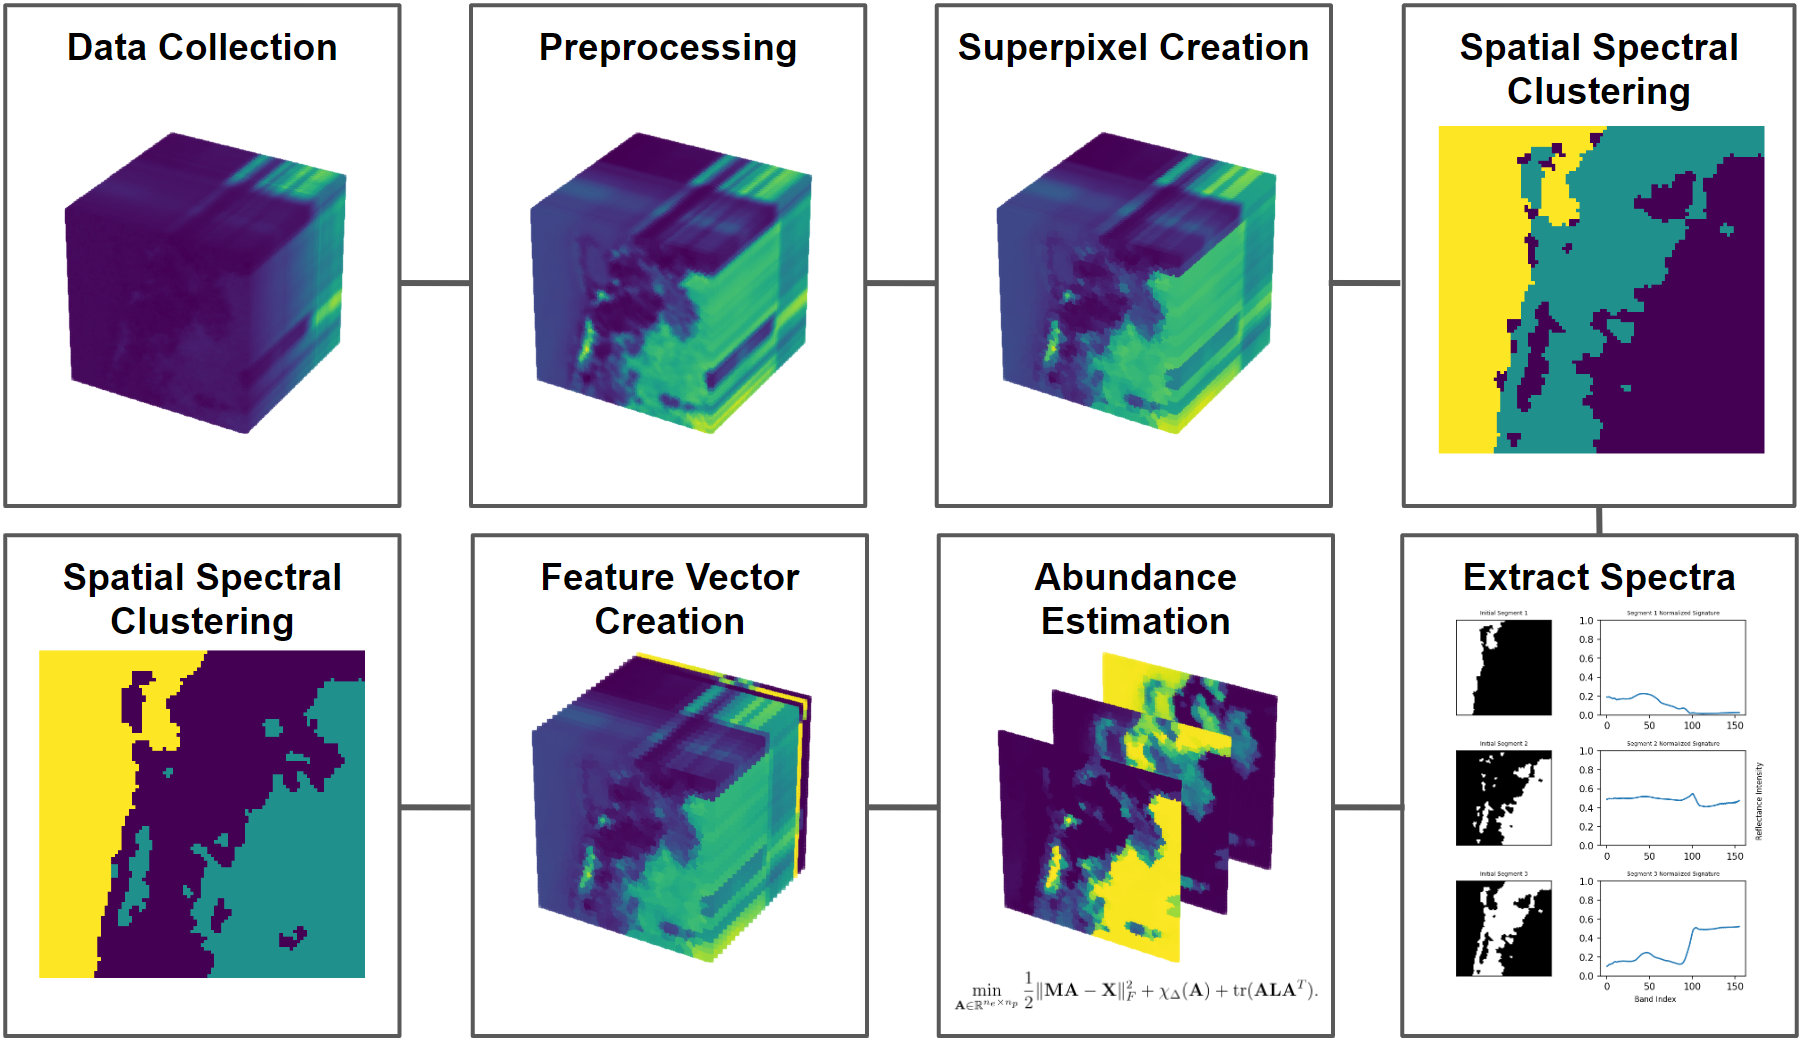
\includegraphics[scale=0.4]{algorithm_view.png}  % Replace filename with your image file name (without extension)
%     \label{fig:label}  % Optional label for referencing the figure in the text
%   \end{figure}
  
